\chapter{XỬ LÝ ADC}
\section{Giới thiệu chung}
\subsection{Yêu cầu}
Đọc giá trị ADC từ biến trở.
\subsection{ADC}
PIC 16F887 có 2 PORT hổ trợ tính năng ADC là: PORT A và PORT E. Có thể đọc ADC ở chế độ $10$ bit $\left({0-1023}\right)$ hoặc $8$ bit $\left({0-255}\right)$ tùy mục đích sử dụng. Điện áp tham chiếu của bộ ADC thường là $5V$.
\subsection{Sơ đồ mạch}
\begin{figure}[!h]
\begin{center}
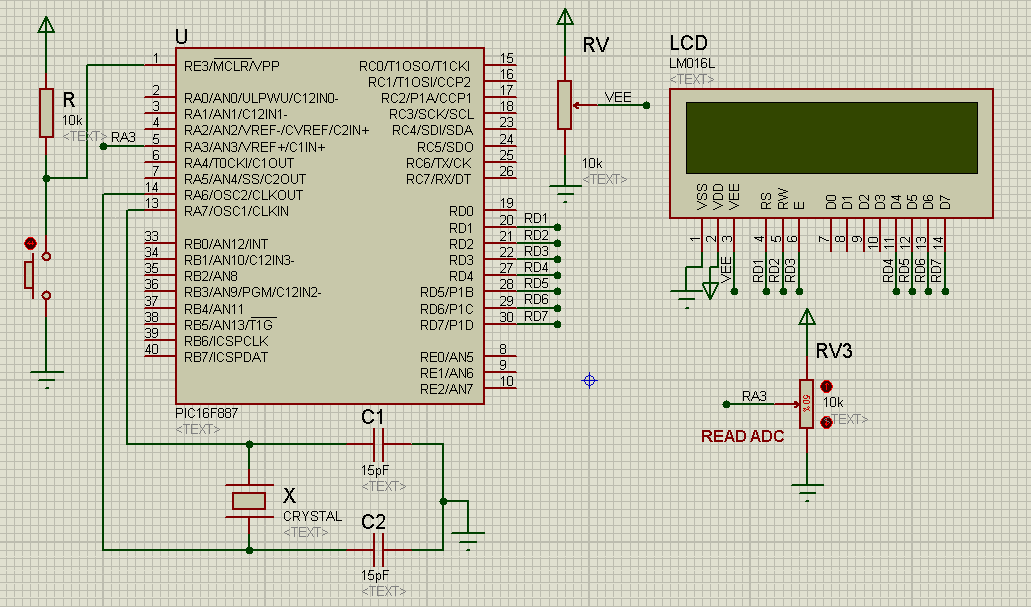
\includegraphics[scale=0.5]{bai-4/image/BAI-4-1}
\end{center}
\caption{Mạch đọc ADC từ biến trở}
\end{figure}
\section{Cấu hình ADC}
\begin{itemize}
\item Khai báo chế độ đọc ADC là $10$ hoặc $8$ bit:

\verb|#DEVICE *= 16 ADC 10| hoặc \verb|#DEVICE *= 16 ADC 8|
\item Xác định cách thức hoạt động của bộ biến đổi ADC: \verb|SETUP_ADC(mode);|
\item Xác định chân lấy tín hiệu ADC và điện thế sử dụng: \verb|SETUP_ADC_PORTS(value);|
%với giá trị của biến \verb|value| ta có thể tham khảo trong phần \verb|Help| của chương trình \verb|CSS|.
\item Chọn chân để đọc Analog với lệnh \verb|READ_ADC|, ta khai báo:

\verb|SET_ADC_CHANNEL(channel);| với \verb|channel| có giá trị từ $0 - 7$ theo tứ tự \verb|A0 - A5; E0 - E2|. Sau hàm này chúng ta nên dùng \verb|delay_us(10)| để cho kết quả đúng.
\item Đọc giá trị ADC từ chân đã khai báo ở hàm \verb|SET_ADC_CHANNEL| với lệnh \verb|READ_ADC(mode);| với \verb|mode| không bắt buộc.
\item[$\ast$] Các tham số (\verb|mode|, \verb|value| và \verb|channel|) của những hàm trên được định nghĩa trong thư mục \verb|DEVICES| ví dụ: \verb|16F887.h|, cách sử dụng những hàm này có thể xem trong phần \verb|Help| của phần mềm CCS.
\end{itemize}
\section{Bài tập}
\subsection{Bài tập 4.1}
\paragraph{Yêu cầu}Viết chương trình đọc giá trị ADC từ biến trở R7 và hiển thị lên LCD.
\paragraph{Hướng giải quyết}
\begin{itemize}
\item Khởi tạo LCD (trình bày trong \emph{chương trình 4 -- bài tập 2.1} của \emph{bài \ref{Les:LCD}}).
\item Cấu hình bộ ADC:
\begin{itemize}
\item Khai số bit đọc ADC, ta chọn \emph{10 bit}: \verb|#device *= 16 ADC 10|
\item Xác định hoạt động của bộ ADC, chọn \emph{thời gian lấy mẫu bằng xung clock}: \verb|SETUP_ADC(ADC_CLOCK_INTERNAL);|
\item Xác định chân đọc ADC, dùng \emph{chân A3}: \verb|SET_ADC_CHANNEL(3);| và \verb|delay_us(10)| (để bảo đảm giá trị đọc chính xác).
\end{itemize}
\item Thực hiện vòng lặp (dùng \verb|while|) đọc giá trị ADC (dùng \verb|READ_ADC|) và cho hiển thị giá trị lên LCD (dùng hàm \verb|printf| kết hợp với hàm \verb|LCD_PutChar|).
\end{itemize}
\newpage
\subsection*{Kết quả}
\begin{figure}[!h]
\vspace{-.5cm}
\begin{center}
  {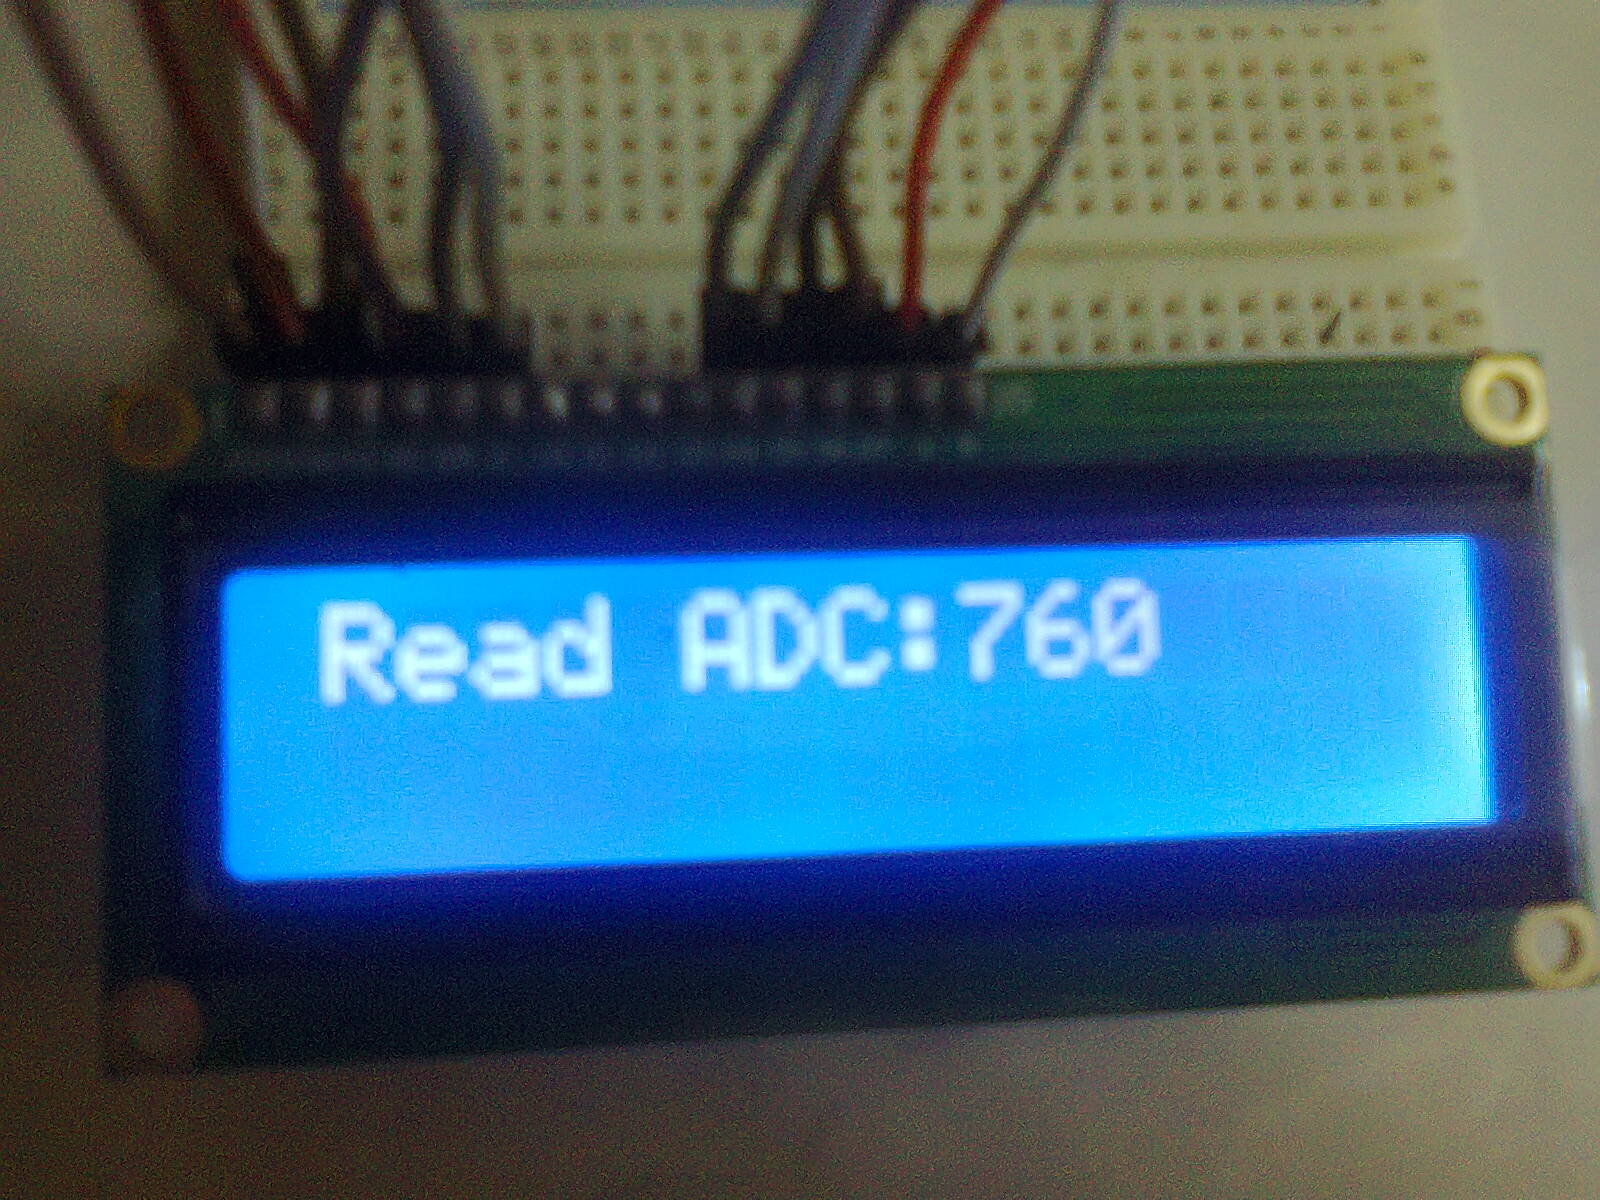
\includegraphics[width=.5\linewidth]{bai-4/image/4-1}}
\end{center}
\caption{Kết quả chương trình ADC hiển thị lên LCD 16x02}
\end{figure}
\subsection*{Chương trình 11}
\lstinputlisting[language=C]{BAI-4-1.C}
\subsection{Bài tập 4.2}
\paragraph{Yêu cầu}Viết chương trình đọc giá trị ADC từ biến trở R7 và xuất ra giá trị các LED ở \verb|PORT E|.
\paragraph{Hướng giải quyết}
\begin{itemize}
\item Đọc giá trị ADC như ở \textit{bài tập 4.1}.
\item Sau khi đọc được giá trị ADC từ biến trở, dùng hàm \verb|OUTPUT_E(value);| với \verb|value| là giá trị ADC đọc được.
\begin{itemize}
\item Giá trị ADC chúng ta đọc được trên LCD là ở dạng số nguyên, nên muốn hiểu rõ trạng thái của LED cần đổi giá trị ADC đọc được sang mã nhị phân.
\item Do \verb|PORT E| chỉ có 3 chân, nên chỉ quan tâm 3 số cuối của mã nhị phân.

Ví dụ: \verb|ADC = 511 = 0b01 1111 1111| (10 bit), chúng ta qua tâm số giá trị cuối của mã nhị phân là \verb|111|, khi đó cả 3 LED đều sáng.
\end{itemize}
\item Viết thêm lệnh chuyển từ số thập phân sang số nhị phân cho hiển thị lên LCD để dễ quan sát.
\end{itemize}
\newpage
\subsection*{Kết quả}
\begin{figure}[!h]
\begin{center}
  {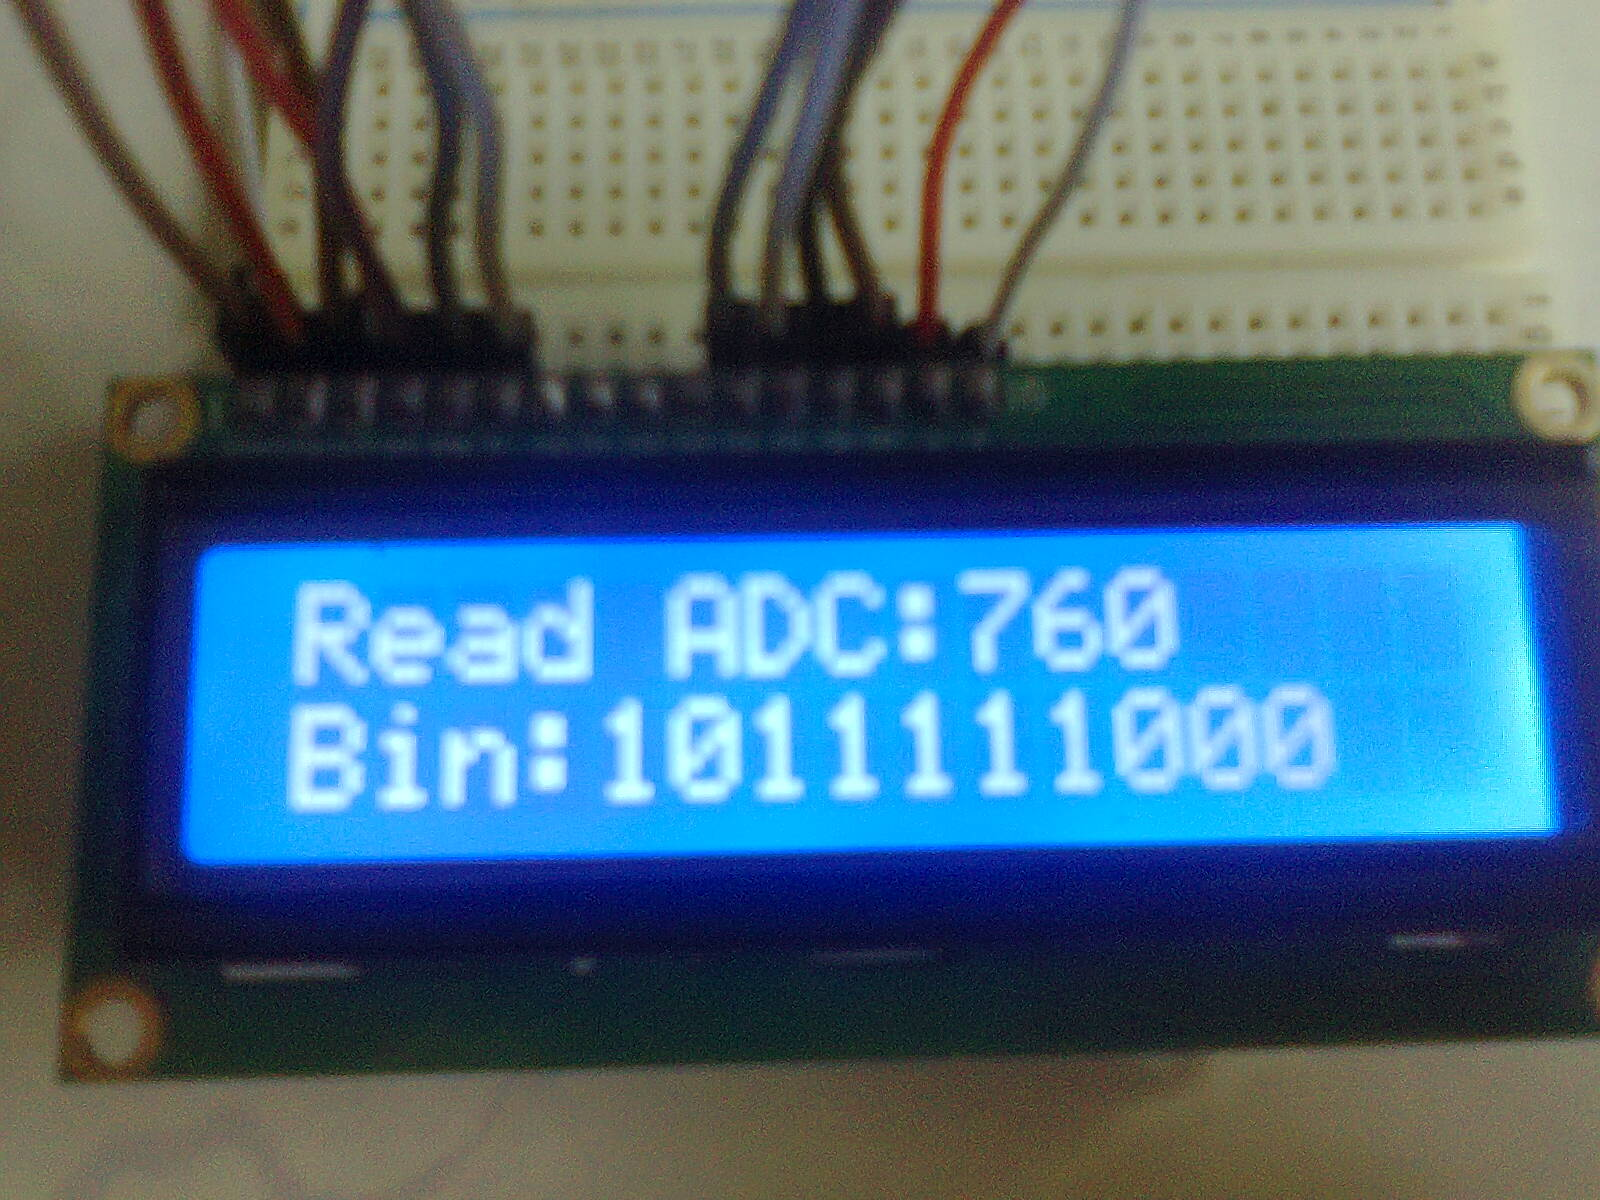
\includegraphics[width=.5\linewidth]{bai-4/image/4-2}}
\end{center}
\caption{Kết quả chương trình ADC xuất ra PORT E}
\end{figure}
\subsection*{Sơ đồ mạch}
\begin{figure}[!h]
\begin{center}
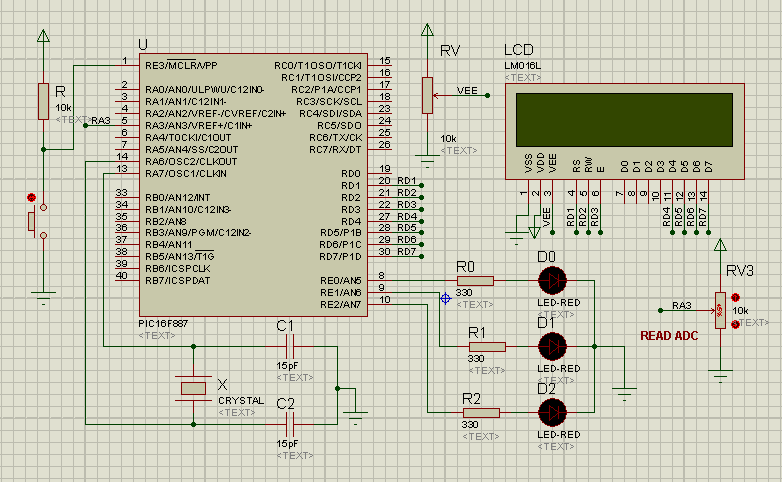
\includegraphics[scale=0.7]{bai-4/image/BAI-4-2}
\end{center}
\caption{Mạch đọc ADC từ biến trở xuất giá trị ra LED}
\vspace{1cm}
\end{figure}
\subsection*{Chương trình 12}
\lstinputlisting[language=C]{BAI-4-2.C}
\subsection{Bài tập 4.3}
\label{Ex:4-3}
\paragraph{Yêu cầu}Viết chương trình đọc ADC từ biến trở và gửi lên máy tính.
\paragraph{Hướng giải quyết}
\begin{itemize}
\item Phần code cho vi điều khiển:
\begin{itemize}
\item Để gửi dữ liệu từ vi điều khiển lên PC, chúng ta sử dụng chuẩn giao tiếp RS232 (được giới thiệu trong \textit{bài \ref{chapter:rs232} trang \pageref{chapter:rs232}}).
\item Thêm vào khai báo sau để giao tiếp RS232:

\verb|#use rs232(baud = 9600, xmit = PIN_C6, rcv = PIN_C7)|
\item Sau khi đọc được giá trị từ biến trở (giống như \textit{bài tập 4.1}), chúng ta gửi dữ liệu lên máy tính bằng lệnh: \verb|printf("%lu",adc)|.
\item Sử dụng lại \textit{chương trình 11} của \textit{bài tập 4.1} cho hiển thị lên LCD để kiểm chứng lại kết quả trên LCD và kết quả gửi lên máy tính.
\end{itemize}
\item Phần code cho Matlab\footnote{Tham khảo tại: http://www.picvietnam.com/forum/showthread.php?t=752}
\begin{itemize}
\item Dữ liệu do vi điều khiển gửi lên máy tính sẽ được lưu trong bộ nhớ đệm, để đọc giá trị từ bộ nhớ đệm ra ta phải thiết lập cho tham số \verb|BytesAvailableFcn|.
\item Khi có một byte được nhận ở bộ nhớ đệm thì tham số này sẽ được gọi.
\item Do đó cần viết hàm (hàm \verb|Serial_Callback| trong file \verb|Serial_Callback.m|) để đáp ứng sự kiện trên và cho hiển thị trực tiếp lên cửa sổ command line.
\end{itemize}
\end{itemize}
\paragraph{Sơ đồ mạch}{~\\}
\begin{figure}[!h]
\begin{center}
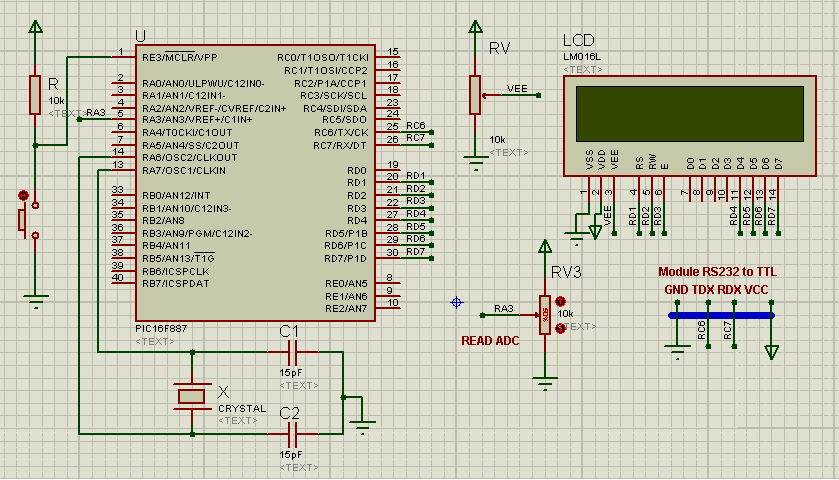
\includegraphics[scale=0.7]{bai-4/image/BAI-4-3}
\end{center}
\caption{Mạch đọc ADC từ biến trở gửi lên PC}
\end{figure}
\subsection*{Chương trình 13}
\lstinputlisting[language=C]{BAI-4-3.C}

Hàm \verb|Serial_Callback| dùng để thiết lập cho tham số \verb|BytesAvailableFcn| trước khi mở cổng COM:
\lstinputlisting[language=Matlab]{Serial_Callback.m}

Lệnh Matlab nhận dữ liệu từ vi điều khiển gửi lên:
\lstinputlisting[language=Matlab]{BAI-4-3.m}